\section{Signalübertragung}
Um digitale Signale zu übertragen in einem Differenzsignal, sollten sich die Energie von Mark (1) Space (0) maximal unterscheiden.
\[
s_2(t) = -s_1(t)
\]

\subsubsection{Unipolar NRZ, NRZ-L}\script{93}
Unipolar Non-Return-To-Zero Leitungscode:\\
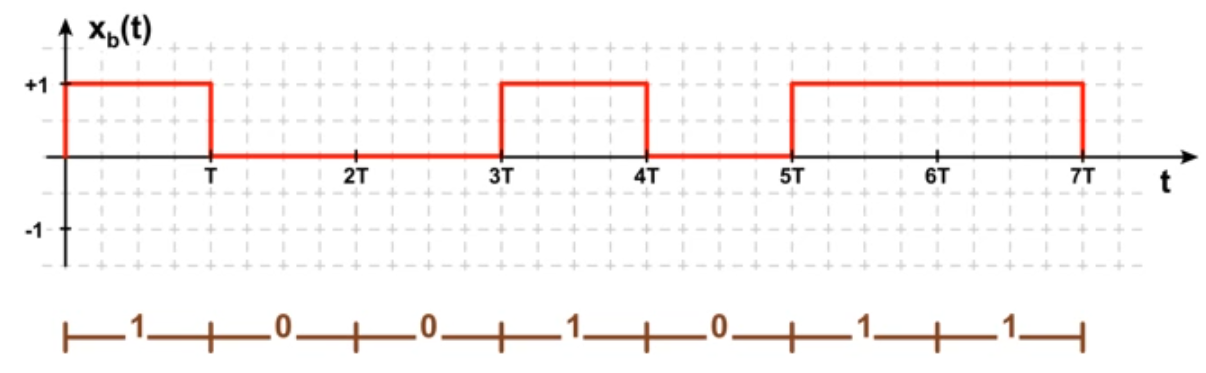
\includegraphics[width=0.6\columnwidth]{Images/nrz}

Verbesserung des NRZ können durch Scrambling, Bitstopen oder 8b/10b-Codierung erreicht werden.

\subsubsection{Bipolar NRZ}\script{95}
Bipolar NRZ Leitungscode:\\
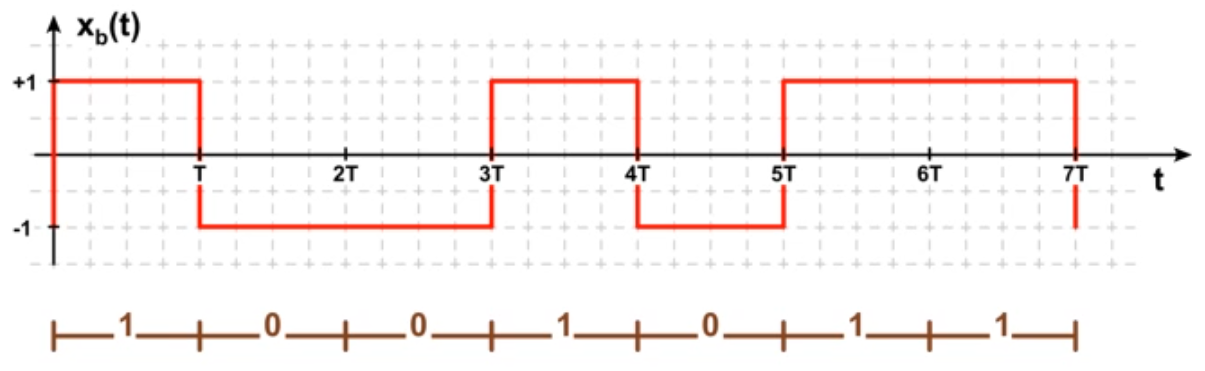
\includegraphics[width=0.6\columnwidth]{Images/nrz1}

\subsubsection{NRZI}\script{96}\\
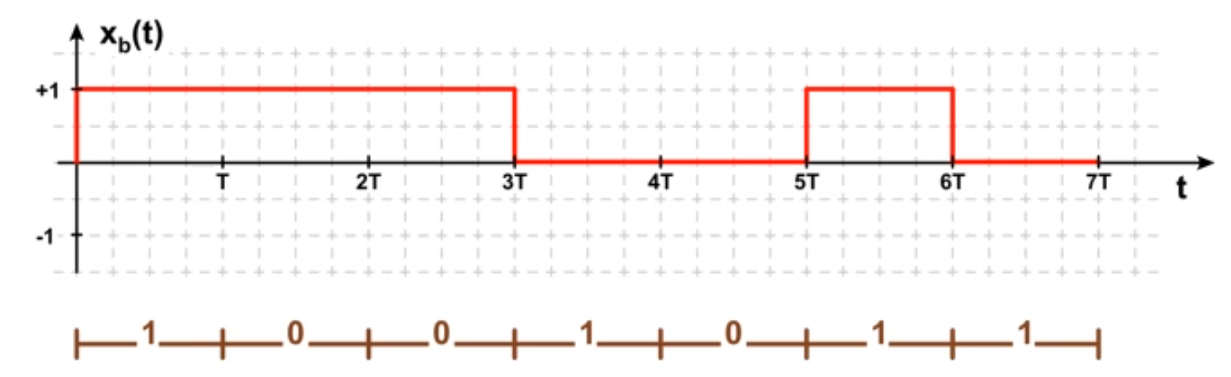
\includegraphics[width=0.6\columnwidth]{Images/nrzi}

\subsubsection{Unipolar RZ}\script{97}\\
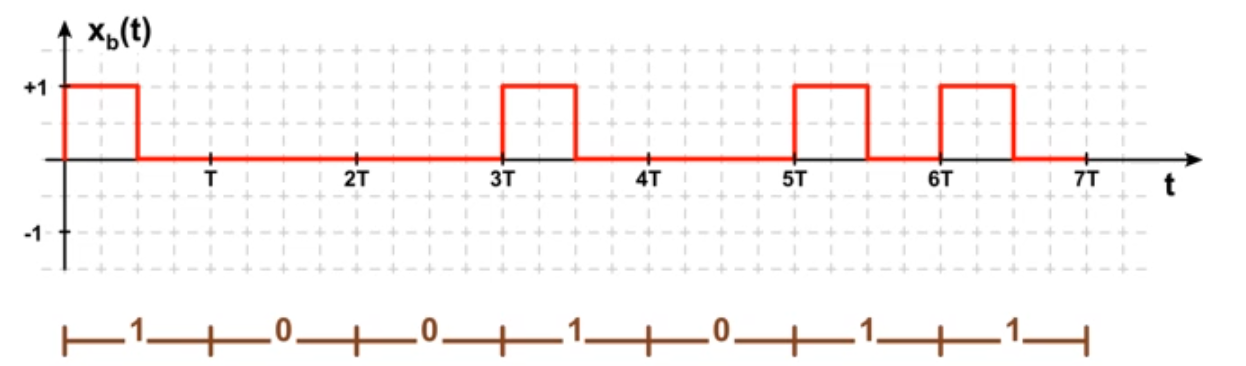
\includegraphics[width=0.6\columnwidth]{Images/urz}

\subsubsection{Bipolar RZ}\script{97}\\
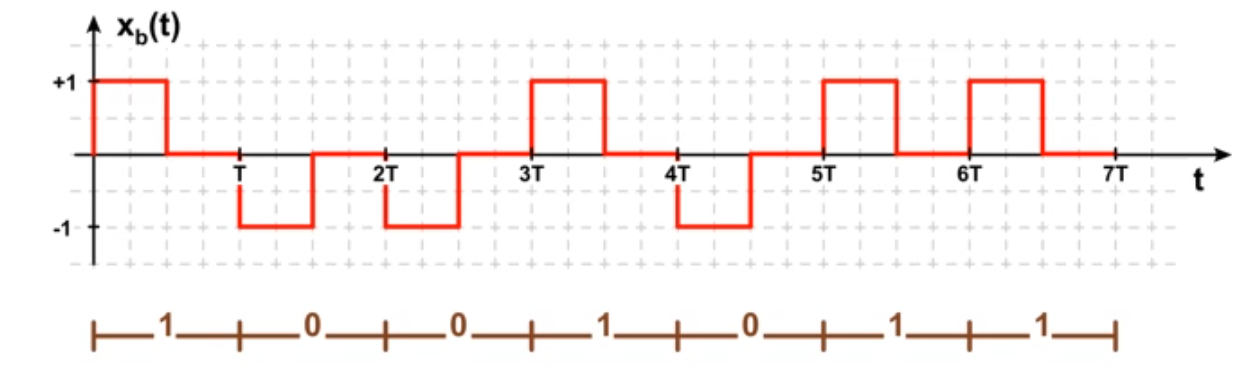
\includegraphics[width=0.6\columnwidth]{Images/brz}

\subsubsection{AMI}\script{98}
Alternative Mark Inversion\\
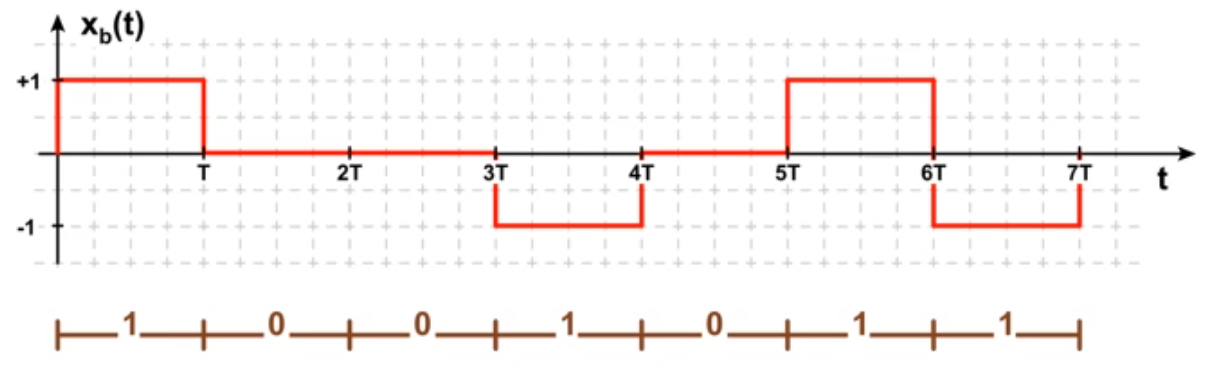
\includegraphics[width=0.6\columnwidth]{Images/ami}

\subsubsection{Manchester Code}\script{99}
Auch Split-Phase, Biphase Level\\
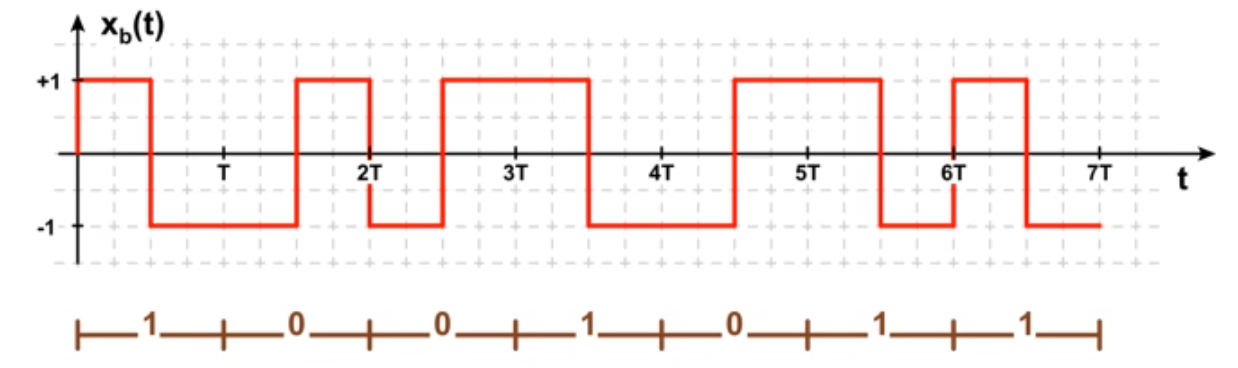
\includegraphics[width=0.6\columnwidth]{Images/manchester}

\subsubsection{MLT3}\script{99}\\
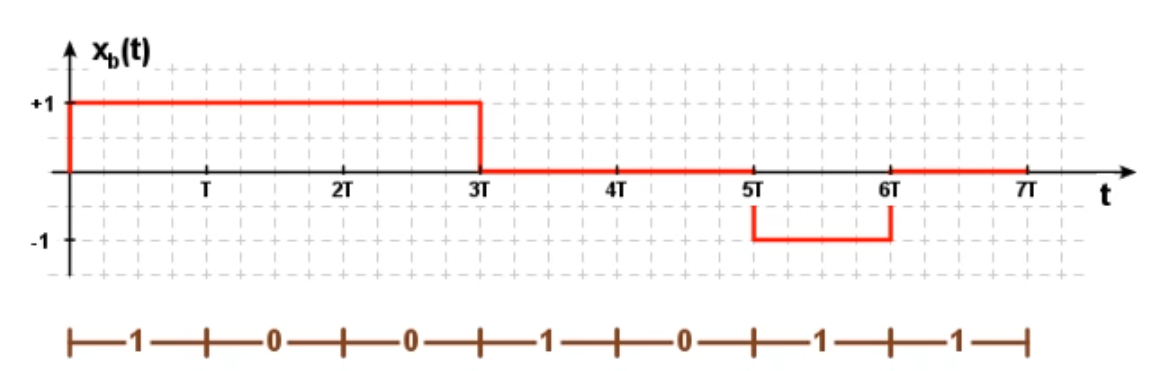
\includegraphics[width=0.6\columnwidth]{Images/mlt3}

\subsubsection{PAM5}\script{101}\\
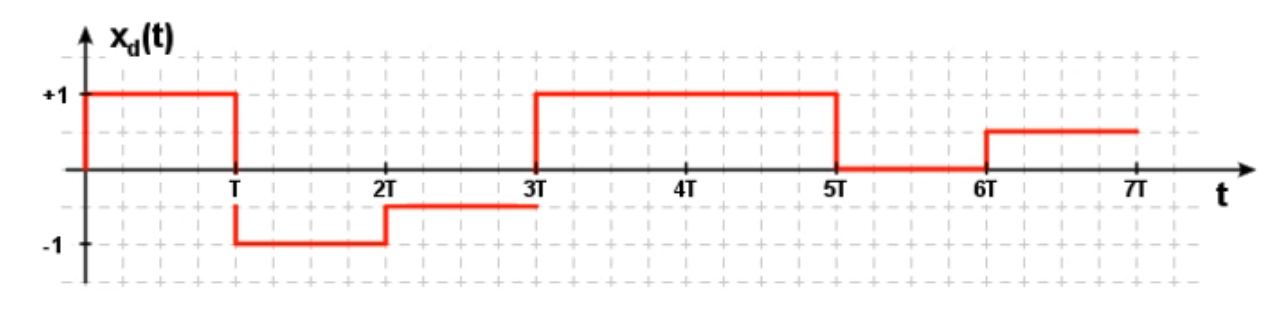
\includegraphics[width=0.6\columnwidth]{Images/pam5}


\subsection{Bandbreitenbedarf}\script{102}
Der minimale Bandbreite $B_d$ [Hz] kann abgeschätzt werden mit $B_d = \frac{f_s}{2}; f_s = \frac{1}{T_s}$

\subsection{Äquivalente Basisbanddarstellung von Bandpasssignalen} \script{114}\\
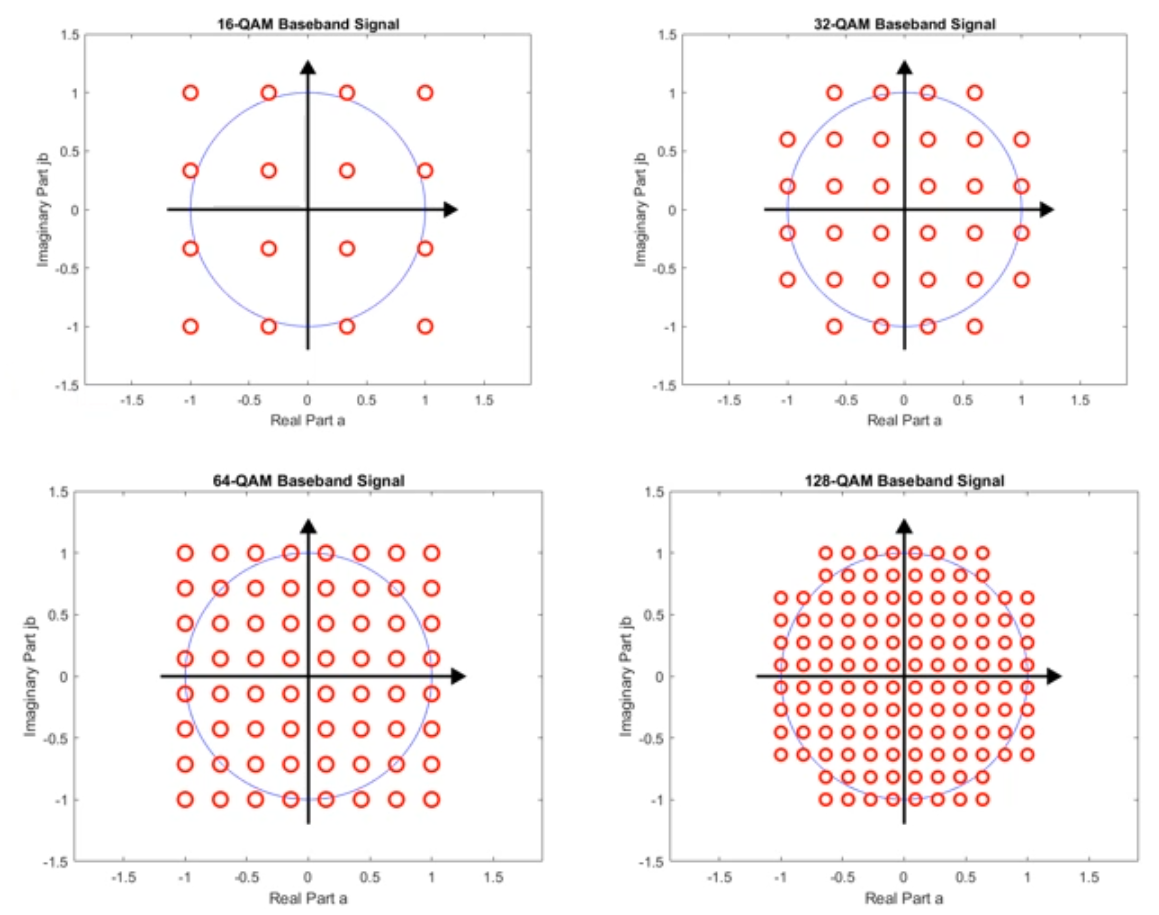
\includegraphics[width=\columnwidth]{Images/qam_basisdarstellung}
